\section{Geld}
Geld erleichtert die Zahlungsvorgänge bei Tauschgeschäften. Als Geld können verschiedene Zahlungsmittel dienen, sofern sie folgende Ansprüche erfüllen.
\begin{itemize}
	\item Tauschmittel: reduziert Transaktionskosten des Kaufprozesses
	\item Wertaufbewahrungsmittel: "Lagerung" von Kaufkraft (ausser bei hoher Inflation)
	\item Masseinheit: Vergleichbarkeit des relativen Wertes von Gütern
	\item ...und Akzeptanz: Dritte müssen bereit sein, das Zahlungsmittel entgegen zu nehmen
\end{itemize}

\subsection{Wer schafft Geld?}
\begin{minipage}{0.6\linewidth}
	\textbf{Entstehung des modernen Bankensystems}
	\begin{itemize}
		\item Gold ist das anerkannte Zahlungsmittel im 15. Jahrhundert.
		\item Besitzer hinterlegen Gold bei Goldschmieden, diese stellen dafür Quittungen aus.
		\item Die Quittungen erhalten Geldcharakter (100\% Golddeckung).
		\item Goldschmiede erkennen, dass über einen längeren Zeitraum nur ein Teil des hinterlegten Geldes abgeholt wird.
		\item Goldschmiede beginnen überproportional viele Quittungen auszustellen und gewähren damit Interessierten Kredite gegen Verzinsung.
		\item Damit werden sie zu Bankiers. Keine 100\% Golddeckung (Geldschaffung), Zahlungsfähigkeit (Fähigkeit zur Rückzahlung) basiert auf Vertrauensbasis ("Fiatgeld").
	\end{itemize}
	\textbf{Geldschöpfung heute im Überblick}
	\begin{itemize}
		\item Die Geschäftsbanken können heute auf der Grundlage des Notenbankgeldes (statt früher Gold) Geld schaffen.
		\item Um das Vertrauen in die Landeswährung zu erhalten ist eine Bankenregulierung notwendig:
		\begin{itemize}
			\item Vertrauen in Zahlungsfähigkeit der Banken!
			\item Mindestreserve-Satz (RS) beschränkt Geldschöpfungspotential der Geschäftsbanken
			\item Geldschöpfungsmultiplikator $GM= 1/RS$ (CH: max. 40)
			\item Nationalbanken beeinflussen die Gesamtgeldmenge (M2) über die Notenbankgeldmenge (M0) und den Geldschöpfungsmultiplikator.
			\item Basispunkt ist absolute Wertangabe.
			\subitem Zins von 1\% auf 2\% Vergrösserung um 1000 Basispunkte
		\end{itemize}
	\end{itemize}
\end{minipage}%
\begin{minipage}{0.4\linewidth}
	\vspace{-12em}
	\fbox{\begin{minipage}{\linewidth}
	Ausgewählte Mindestreserve-Sätze 2018:
	\begin{itemize}
		\item{\makebox[1.5cm]{EZB\hfill}} 1\%
		\item{\makebox[1.5cm]{Schweiz\hfill}} 2.5\%
		\item{\makebox[1.5cm]{USA\hfill}} 10\%
		\item{\makebox[1.5cm]{China\hfill}} 20\%
	\end{itemize}
	\end{minipage}}\\
	\begin{itemize}
		\item \textbf{M0}
		\subitem Geldschöpfung der Zentralbank (SNB)
		\subitem Offenmarktpolitik
		\subitem theoretisch unbeschränkt
		\item \textbf{M1, M2, M3}
		\subitem Geldschöpfung der Geschäftsbanken
		\subitem Kreditvergabe
		\subitem beschränkt durch Mindestreservesatz
	\end{itemize}
	\vfill
\end{minipage}


\subsection{Geldmengenaggregate in der Schweiz}
\begin{multicols}{2}
	\begin{itemize}
		\item Notenbankgeldmenge \textbf{M0}
		\subitem Noten (Bargeldumlauf) + Girokonten der Geschäftsbanken bei der SNB
		\item Geldmenge \textbf{M1}
		\subitem M0 + Sichteinlagen und Transaktionskosten bei Geschäftsbanken (für Zahlungszwecke)
		\item Geldmenge \textbf{M2}
		\subitem M1 + Spareinlagen bei Geschäftsbanken
		\item Geldmenge \textbf{M3}
		\subitem M2 + Termineinlagen bei Geschäftsbanken (fälligkeitsgebunden)
		\item Die Geschäftsbanken verfügen über ein Girokonto bei der Nationalbank, dort können sie Geld mit Zinszuschlag kaufen
		\item Das erfundene Geld der Nationalbank ist Fremdkapital, weil die Girokonten den Geschäftsbanken gehören
		\item Die Geschäftsbanken können aber auch Geld bei anderen Banken zum Liborzins kaufen.
	\end{itemize}
	\vfill\null
	\columnbreak
	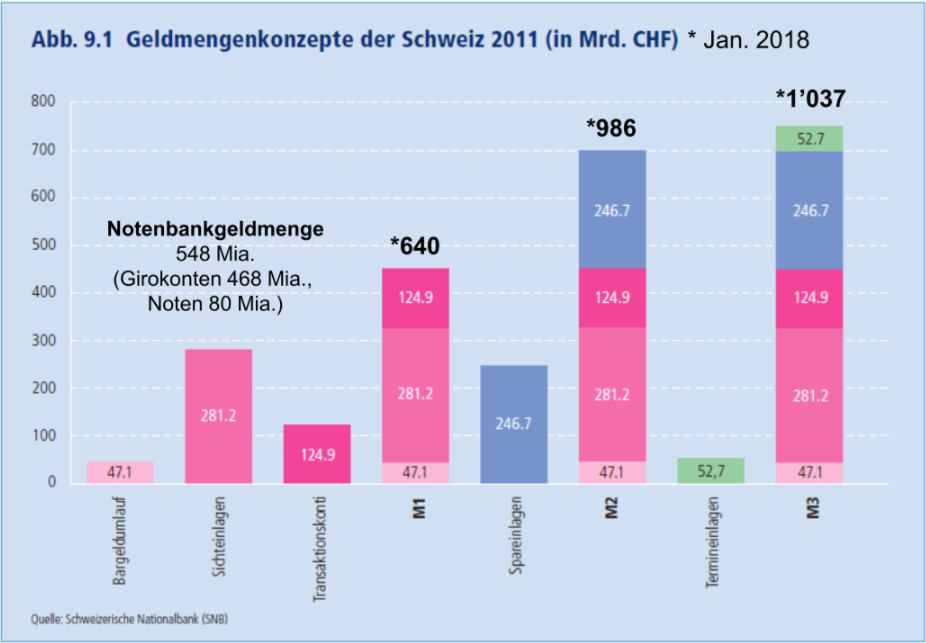
\includegraphics[width=\linewidth]{images/geldmengen.png}
\end{multicols}

\subsection{Funktion der Girokonten}

\subsubsection{Zahlungsverkehr}
\begin{itemize}
	\item SNB
	\begin{itemize}
		\item Systemmanagerin
		\item Auftraggeberin
		\item Zuständigkeit:
		\begin{itemize}
			\item Festlegung Teilnehmerkreis/Teilnahmevoraussetzungen
			\item Führen von Giro-/Verrechnungskonten
			\item Erlass von Abwicklungs-/Verhaltensregeln
			\item Monitoring/Steuerung des Systems
			\item Bereitstellung von Liquidität für Abwicklung
			\item Organisation Krisenmanagement, Leitung Krisenstab SIC
		\end{itemize}
	\end{itemize}
	\item[\-] $\uparrow$
	\item SIC-Vertrag: Ein grosser Teil des Schweizerischen Zahlungsverkehrs findet über Swiss Interbank Clearing SIC statt. Dazu dienen unter anderem die Girokonten der Finanzintermediären.
	\item[\-] $\downarrow$
	\item SIX Interbank Clearing AG
	\begin{itemize}
		\item Betreiberin
		\item Zuständigkeit
		\begin{itemize}
			\item technische Überwachung Tagesbetrieb
			\item Softwareentwicklung/-wartung
			\item Verwaltung Datenbestände
			\item Entwicklung/Betreuung admin. Verhaltensregeln
			\item Betrieb IT-Infrastruktur
		\end{itemize}
	\end{itemize}
\end{itemize}
Geschäfte zwischen den Finanzintermediären (Geschäftsbanken) beeinflussen die Geldmenge nicht, lediglich Geschäfte zwischen der SNB und den Finanzintermediären.

\subsubsection{Liquidität}
\begin{multicols}{2}
	Die Geschäftsbanken können Geld bei der SNB zum SARON plus Zinszuschlag "kaufen".\\
	Eine weitere Möglichkeit ist der Kauf von Schweizer Geld bei anderen Geschäftsbanken in London zum LIBOR-Satz.
	\vfill\null
	\columnbreak
	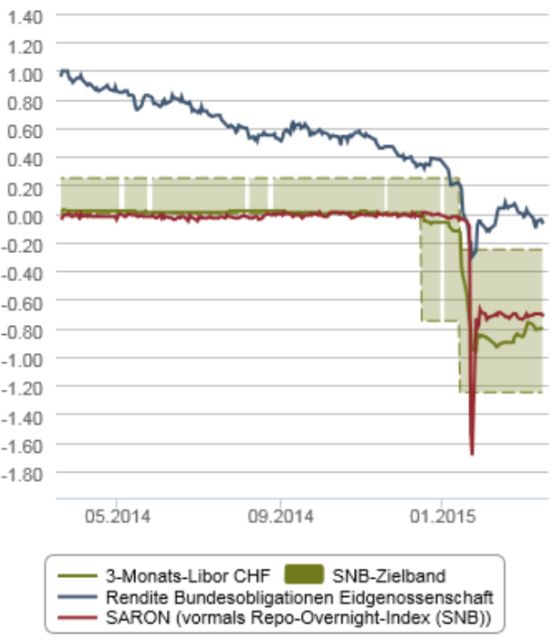
\includegraphics[width=0.5\linewidth]{images/libor.png}
\end{multicols}

\subsection{Bilanz der SNB}
\includegraphics[width=18cm]{images/snb.jpg}
\begin{multicols}{2}
	\begin{description}
		\item[Aktiva] Mittelverwendung
		\subitem Andere Aktiva: SNB kauft keine Währungen!
		\item[Passiva] Mittelherkunft
	\end{description}
	SNB macht Geld um Sachen zu kaufen $\rightarrow$ schöpft Geld\\
	SNB verkauft Sachen $\rightarrow$ zerstört Geld
	\vfill\null
	\columnbreak
	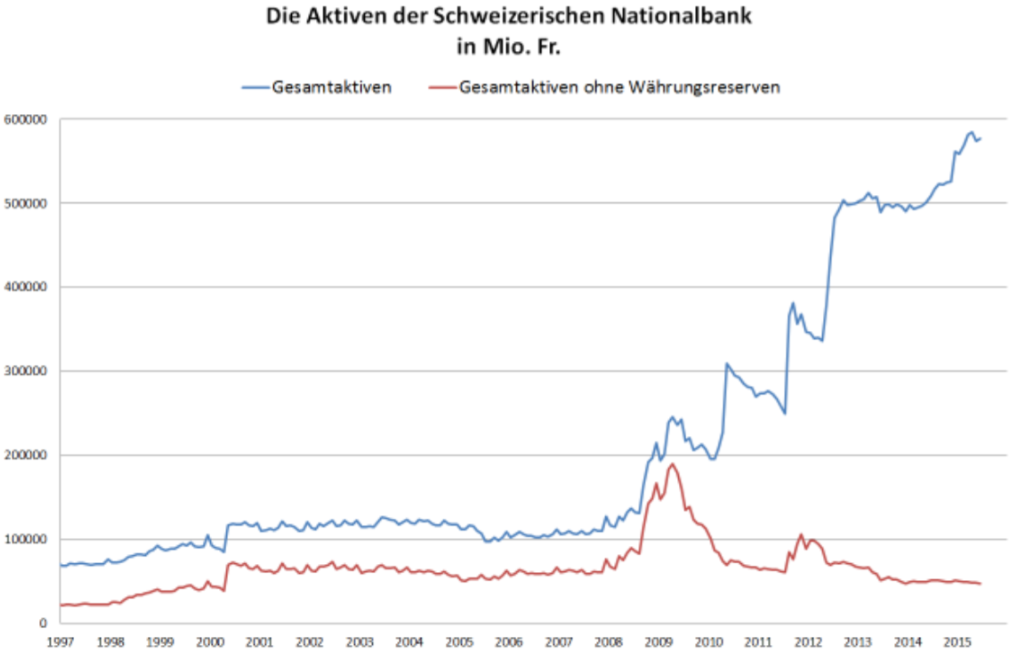
\includegraphics[width=\linewidth]{images/aktiven.png}
\end{multicols}

\subsection{Instrumente der Geldpolitik}

\subsubsection{Offenmarktpolitik}
\begin{enumerate}
	\item Kauf und Verkauf von Aktiva (vor allem Wertschriften) durch SNB bei inländischen Geschäftsbanken
	\begin{itemize}
		\item Nationalbank bezahlt mit $"$frischem gedrucktem$"$ Geld (erfunden), welches auf die Girokonten gutgeschrieben werden.
		\item Kauf von Aktiva ist i.d.R ein Repogeschäft, d.h. der Verkäufer verpflichtet sich zum späteren Rückkauf (also ein gesicherter Kredit mit Zins; früher Repo-Zinssatz, seit 2009 SARON mit Zinszuschlag; Swiss Average Rate Overnight)
	\end{itemize}
	\item Ausgabe von eigenen Schuldverschreibungen (SNB Bills) $\rightarrow$ damit wird Liquidität gebunden
\end{enumerate}

\subsubsection{Mindestreservepolitik}
\begin{itemize}
	\item Nationalbank kann den Mindestreservesatz für Geschäftsbanken festlegen $RS = \frac{1}{GM}$
	\item Damit wird der Geldschöpfungsmultiplikator beeinflusst.
\end{itemize}

\subsubsection{Negativzinsen auf Giroguthaben}
\begin{multicols}{2}
	Finanzintermediäre wie Vermögensverwalter, Versicherungen und Pensionskassen haben keine Mindestreserve-Erfordernis, d.h. ihre Freigrenze liegt deutlich tiefer als bei den Geschäftsbanken $\rightarrow$ zahlen auf gesamtes Vermögen Negativzinsen, Banken hingegen zahlen nur auf Vermögen über dem Zwanzigfachen der Mindestreserven (schwarze Linie) Negativzinsen
	\vfill\null
	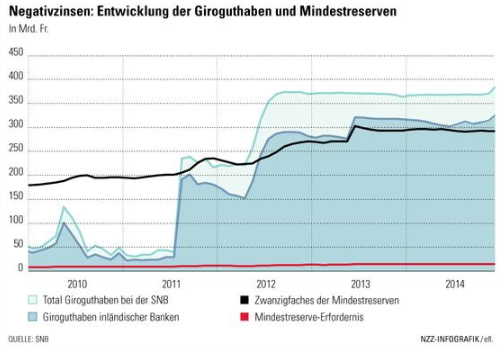
\includegraphics[width=\linewidth]{images/negativzinsen.png}
\end{multicols}

\subsection{Geldpolitische Strategien}
Mögliche Zielsetzungen der Geldpolitik:
\begin{itemize}
	\item \textbf{Wechselkursziele}
	\begin{itemize}
		\item Fixierung des Wechselkurses an internationale Leitwährung
		\item Gefahr eines Importes von Inflation
	\end{itemize}
	\item \textbf{Geldmengenziele}
	\begin{itemize}
		\item{\makebox[4.5cm]{Monetaristischer Ansatz\hfill}} $P \cdot Q = M \cdot V$
		\item{\makebox[4.5cm]{Liquiditätsfalle\hfill}} $P \cdot Q = M\uparrow \cdot V \downarrow$ \qquad $\rightarrow$ funktioniert nur solange V konstant ist!
	\end{itemize}
	\item \textbf{Inflationsziele}
	\begin{itemize}
		\item Wahrung der Preisstabilität
	\end{itemize}
\end{itemize}

\subsection{Schweizer Geldpolitik}

\subsubsection{Mandat der SNB}
\begin{itemize}
	\item Vorrangiges Ziel ist die Preisstabilität und nachrangig die Berücksichtigung der Konjunktur (gemäss Verfassung und Gesetz)
	\item Unabhängigkeit vom Staat; Bundesrat hat keine Weisungsbefugnisse gegenüber der SNB
\end{itemize}
Die Nationalbank hat in Bern und Zürich je einen Sitz. Daneben unterhält sie Vertretungen in Basel, Genf, Lausanne, Lugano, Luzern und St. Gallen. Dazu kommen 14 Agenturen, die von Kantonalbanken geführt werden und der Geldversorgung des Landes dienen.\\
Die Nationalbank ist eine spezialgesetzliche AG des Bundesrechts. Sie wird unter Mitwirkung und Aufsicht des Bundes nach den Vorschriften des Nationalbankengesetzes verwaltet. Die Aktien sind als Namenpapiere ausgestaltet und an der Börse kotiert. Das Aktienkapital beträgt 25 Millionen Franken und ist zu rund 55\% im Besitz der öffentlichen Hand (Kantone, Kantonalbanken etc.). Die übrigen Aktien befinden sich grösstenteils im Besitz von Privatpersonen. Der Bund besitzt keine Aktien. Sie ist mit 600 Mitarbeitenden eine der kleinsten Zentralbanken in Europa.

\subsubsection{Historische Entwicklung}
\textbf{1945-1973: Orientierung am Wechselkurs}\\
\begin{itemize}
	\item Teilnahme der Schweiz am Bretton-Woods-System (fixe Wechselkurse)
	\item US-Dollar als internationale Leitwährung
	\item Finanzierung des Vietnamkriegs (Ausweitung der US-Geldmenge) führt zu importierter Inflation in vielen Ländern
	\item Golddeckung in den USA nahm massiv ab, deshalb Aufkündigung der Goldeinlösungspflicht durch US-Regierung
	\item Zusammenbruch des Bretton-Woods-Systems
\end{itemize}
\vspace{\baselineskip}
\textbf{1974-1999: Orientierung an der Geldmenge}
\begin{itemize}
	\item Ausrichtung am Monetarismus (Ökonomische Theorie, dass Inflation immer durch ein Überangebot an Geld verursacht wird)
	\item Ende 80er-Jahre viele Innovationen auf dem Finanzmarkt mit Einfluss auf die Umlaufgeschwindigkeit des Geldes
	\item Häufigeres Verfehlen der Geldmengenziele
\end{itemize}
\vspace{\baselineskip}
\textbf{Seit 1999: Orientierung an Inflationsprognosen}
Inflationsprognosen anhand der Geldmengen M2 und M3 (SNB kommuniziert diese Indikatoren im Gegensatz zur EZB allerdings nicht)\\
Umsetzung mit folgendem geldpolitischen Konzept:
\begin{enumerate}
	\item Definition der Preisstabilität (Ziel)
	\item Inflationsprognose (Entscheidungsgrundlage)
	\item Zielband für Dreimonats-Libor (operatives Ziel)
\end{enumerate}

\subsection{Krypto-Währungen}
Krypto-Währungen sind dezentrale Währungen. Der Bitcoin ist mit einem Gesamtwert aller sich im Umlauf befindlichen Coins von 16467 Mio. US-Dollar die "erfolgreichste" Krypto-Währung. Weitere sind Ethereum (749 Mio.), Ripple (229 Mio.), Litecoin und Monero (je 225 Mio.) usw.

\subsubsection{Bitcoin}
\begin{itemize}
	\item neuartige Form von elektronischem Geld
	\item wird dezentral durch eine Computernetz geschöpft und verwaltet
	\item erfüllt klassische Geldfunktionen: Tausch, Messung und Wertaufbewahrung
	\item Bitcoin-Einheiten sind durch starke Verschlüsselungsverfahren fälschungssicher
	\item jeder Geldbetrag kann nur einmal ausgegeben werden, weil jede Übermittlung im Netzwerk verzeichnet wird
	\item schnelle Bestätigung von Transaktionen (10-60 Minuten)
	\item geringe Kosten pro Transaktion
	\item Besitz von Beträgen wird durch Inhalt einer elektronische Geldbörse nachgewiesen, welche kryptographische Schlüssel enthält
	\item Jedes Bitcoin lässt sich in 100 Mio. Einheiten unterteilen (kleinste Einheit = "Satoshi")
\end{itemize}
\vspace{\baselineskip}
\textbf{Meilensteine}
\begin{itemize}
	\item Konzept wurde 2008 von Satoshi Nakamoto (Pseudonym) vorgeschlagen
	\item Netzwerk entstand 2009
	\item Bitcoins hatten anfangs keinen in anderen Währungen bezifferbaren Wert
	\item 2010 wurden erste Wechselkurse durch Personen in "bitcointalk"-Foren ausgehandelt
\end{itemize}
\begin{multicols}{2}
	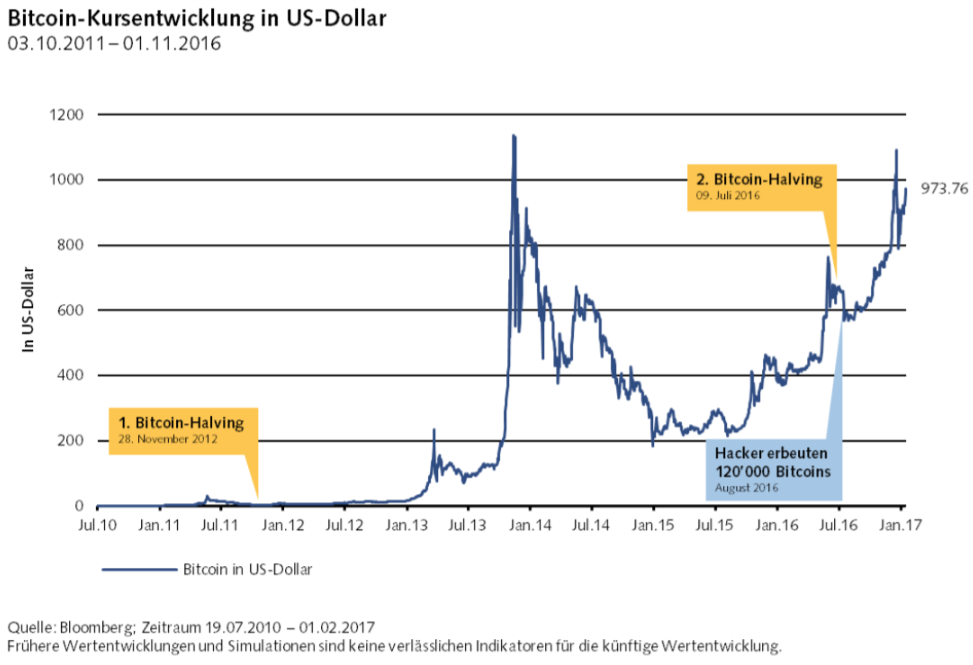
\includegraphics[width=\linewidth]{images/bitcoin1.png}
	\columnbreak
	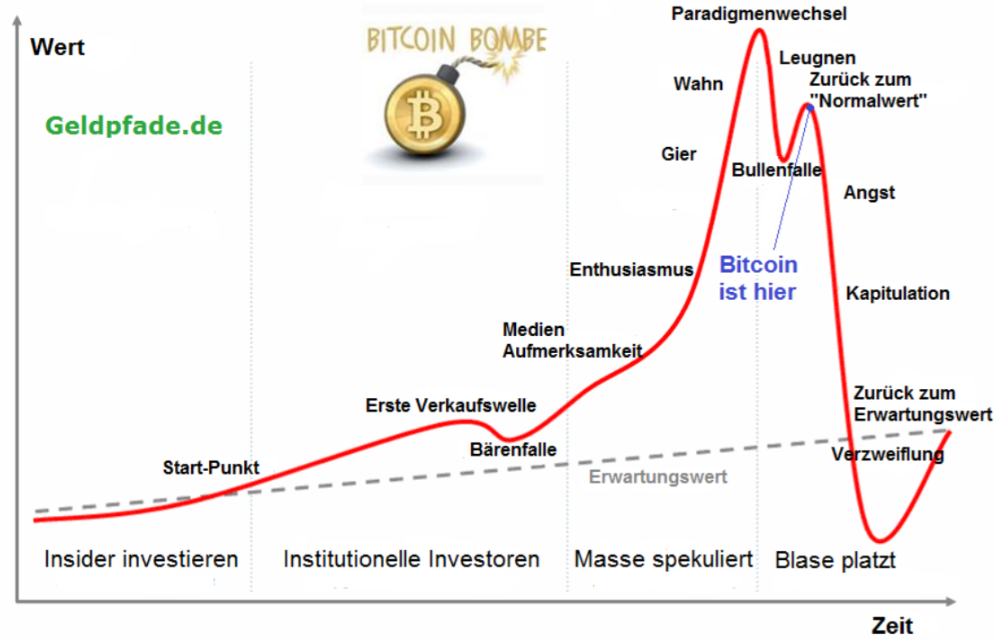
\includegraphics[width=\linewidth]{images/bitcoin2.png}
\end{multicols}
\begin{minipage}{0.5\linewidth}
	\textbf{Schöpfung von Bitcoins: Wer stellt den Wert von Bitcoins sicher?}\\
	Bitcoin hat die Eigenschaft einer begrenzten Geldmenge. Die maximale Menge an Bitcoins wurde beim Entwurf des Bitcoin-Protokolls auf 21 Mio. festgelegt (wird voraussichtlich 2033 erreicht).\\
	Neue Bitcoin-Einheiten werden nach einem Prinzip verteilt, das die Unterstützung des Netzwerks durch Zur-Verfügung-stellen von Rechenleistung belohnt (Bitcoin-"Mining").\\
	Vor einem Bezahlvorgang muss der Nutzer Bitcoins erarbeiten oder kaufen.
\end{minipage}
\begin{minipage}{0.45\linewidth}
	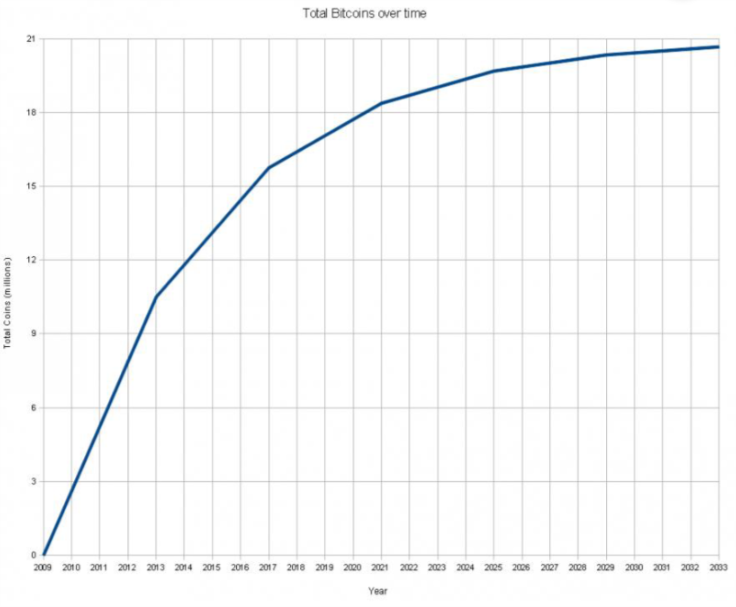
\includegraphics[width=\linewidth]{images/bitcoin3.png}
\end{minipage}

\clearpage
\pagebreak